\nfch{Part 1}{Sublinear Explicit}{Incremental Voronoi Diagrams}
\def\paw{paw } \def\paws{paws } \def\Ot{\tilde O}

\def\animSlide#1#2{
\begin{frame} \frametitle{Voronoi Diagram: basics} \vspace{-7mm}

\begin{block}{\vspace*{-3ex}}
Voronoi diagram of $S = \{ s_1, \ldots, s_N \}$:
     subdivision of the Euclidean plane,\\
     for each $q$ inside the {\it cell} of $s_i$ \\ \medskip
\centerline{$\mathrm{dist} (q, s_i) < \mathrm{dist} (q, s_j),\quad j\ne i$.}
\end{block}

\begin{figure}[h] \centering
\begin{subfigure}[b]{0.46\textwidth} \centering
	\includegraphics[width=4.9cm]{#1}
	\label{fig:voronoiCircle}
\end{subfigure} ~~
\begin{subfigure}[b]{0.44\textwidth} \centering
	\includegraphics[width=4.7cm]{#2}
	\label{fig:Paw}
\end{subfigure}
\end{figure} \end{frame}
}

\animSlide{figs/voronoiDiagram}{figs/nCell}
\animSlide{figs/voronoiCircle}{figs/nCell}
\animSlide{figs/voronoiCircle}{figs/neighbor}

\begin{frame} \frametitle{Dynamic VD: setting}
\begin{block}{Incremental Voronoi Diagram}
	Maintain initially empty Voronoi diagram under insertion of new sites
\end{block} \smallskip

	There is a linear-time solution, no faster solutions possible: there may be \\
	$O(N)$ changes per insertion. \bigskip \pause

\begin{block}{Incremental Combinatorial Voronoi Diagram}
	Maintain the graph of initially empty Voronoi diagram under insertion of new sites
\end{block} \smallskip

	There is a naive linear-time algorithm. Can we find a faster solution?
\end{frame}

\begin{frame} \frametitle{Dynamic VD: combinatorial changes}
\vspace{2mm}
\begin{theorem}[\acite{incremental-vd}]
\label{thm:amorCost} \small
	The number of cells with combinatorial changes is $O(N^{\frac12})$ amortized, there are a constant number of combinatorial changes per cell, cells with changes are connected.
\end{theorem} \medskip \pause

When we are inserting new site $s_N$, the graph of the VD undergoes \\
operation called {\it flarb.} \vspace{-4mm}

\begin{figure}[h]
\centering
	\begin{subfigure}[t]{0.28\textwidth}
	\centering
	\includegraphics[width=3.8cm]{flarb/2flarb}
	\caption{Graph before flarb}
	\label{fig:flarb}
	\end{subfigure}
~
	\begin{subfigure}[t]{0.28\textwidth}
	\centering
	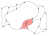
\includegraphics[width=3.8cm]{flarb/3afterflarb}
	\caption{Graph after flarb}
	\label{fig:afterflarb}
	\end{subfigure}
~
	\begin{subfigure}[t]{0.37\textwidth}
	\centering
	\includegraphics[width=4.4cm]{figs/identFlarb}
	\caption{Flarb on a VD}
	\label{fig:afterflarb}
	\end{subfigure}
\label{fig:exflarb}
\end{figure} \end{frame}

\begin{frame} \frametitle{Identifying changes}
\begin{tabular}{lcl}
\makecell[l]{
    \textcolor{hard}{\bf Theorem:} Let $g$ be a cell adjacent to $f$. \\
    Cell $g$ needs to undergo changes $\Longleftrightarrow$ \\
    circle of either of its vertices that are \\
    paws of $f$ encloses $s_N$.\qquad\acite{incremental-vd}
} & \qquad
& \makecell[c]{
	\includegraphics[width=5.4cm]{figs/identChanges}
} \end{tabular} \bigskip \pause

\begin{block}{{\it Dynamic circle reporting} structure
	     (\acite{DBLP:journals/jacm/Chan10,incremental-vd})}
	Returns all $k$ circles enclosing given point in $\Ot(k)$. Addition and deletion of \\
	a circle in $\Ot(1)$.
\end{block}
\end{frame}